
\section{Experimentation}
\label{sec:experimentation}

% \TODO{Define what we want.} We measure the time between the broadcast of a
% message and its delivery by all processes in the network. We expect that our
% measurements slowly increase as the network becomes more dynamic.

In this section, we evaluate the impact of \CBROADCAST on the message delivery
in a specific overlay network that corresponds to random graphs. The experiments
run on the \PEERSIM simulator~\cite{montresor2009peersim} that allows
simulations to reach high scale in terms of number of processes. Our
implementation is available on the Github
platform\footnote{\url{http://github.com/chat-wane/peersim-pcbroadcast}}.


\noindent \textbf{Objective:} To observe the transmission delay introduced by
\CBROADCAST on message delivery. We expect the delay to increase as the latency
increase.

\noindent \textbf{Description:} We build an overlay network with a topology
close to random graphs using \SPRAY~\cite{nedelec2017adaptive}. Networks
comprises 1k processes. The network is dynamic. Each process' neighborhood $Q$
changes at least once every 60 seconds. Each exchange involve two processes that
both add and remove half of their partial view.  Links are FIFO, bidirectional,
and have transmission delays. The delay increases over time, i.e., the delay for 
a link to be acknowledged increases during the experiment.\\
We measure the shortest path length from a random set of processes to all other
processes. It represents the time taken by broadcast messages before being
delivered by processes.

\begin{figure*}
  \begin{center}
    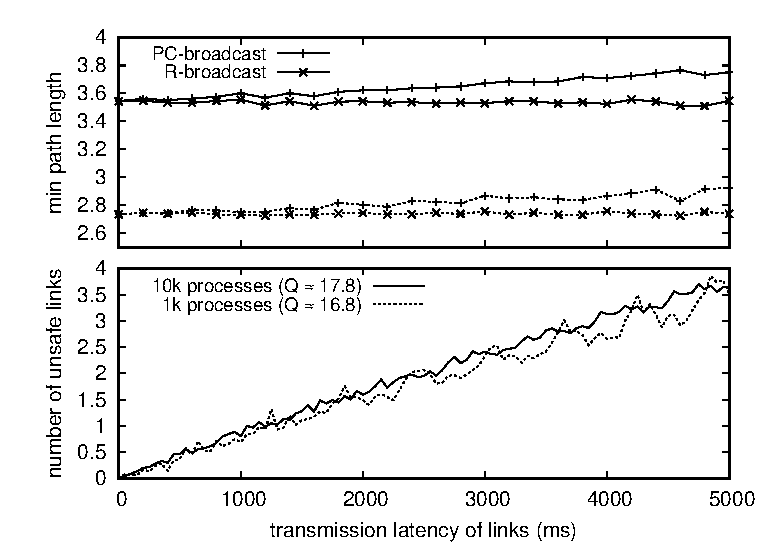
\includegraphics[width=1.4\columnwidth]{./img/delay.eps}
    \caption{\label{fig:delay}Delay in message delivery introduced by \CBROADCAST.}
  \end{center}
\end{figure*}

\noindent \textbf{Results:} Figure~\ref{fig:delay} shows the result of the
experiment. The y-axis depicts the delay set on message transmission for each
link. The top part of the figure shows the average minimal path length. The
bottom part of the figure shows the number of unsafe links that cannot be used 
for causal broadcast yet.
\begin{itemize}[leftmargin=*]
\item Figure~\ref{fig:delay} shows that both R-broadcast and \CBROADCAST deliver
  message quickly to all processes. The overlay network guarantee that paths
  stay short and logarithmically scaling with the number of random neighbors in
  partial views.
\item The top part of Figure~\ref{fig:delay} shows that measurements made on
  \CBROADCAST increases while measurements made on R-broadcast stay
  constant. R-broadcast uses all neighbors provided by \SPRAY while \CBROADCAST
  excludes links still in buffering phase. The more latency on transmission, the
  longer the buffering phase. The bottom part of Figure~\ref{fig:delay} shows
  that the number of elements in the buffers increases accordingly.
\item Figure~\ref{fig:delay} shows that the growth of path length stays small
  even when transmission delays become high. The number of elements in buffers
  stays small because the buffering phase takes a constant number of hops to
  complete: at most 3 hops. The path length grows even slower, for removing 3
  among 17 links has restricted impact on overlay networks close to random
  graphs.
\end{itemize}

This experimentation shows that even under bad network conditions (high
transmission delays) and using highly dynamic overlay networks (random peer
sampling), the number of unsafe links remains small. The negative impact
expected on transmission time before message delivery remains small. In
practice, we expect smaller network transmission delays, and overlay networks
less subject to neighborhood changes (e.g. exploiting user preferences, or
geolocalisation). In such settings, we expect \CBROADCAST to have a negligible
negative impact on the overlay network properties. 

It is worth noting that \CBROADCAST and reactive approaches (\REF) both
introduce delays in message transmission. The former because it cannot use part
of its links for a short time. This is the result highlighted by this experiment
section.  The latter because it overloads messages with control information the
size of which scale linearly with the network size (e.g. each message convey a
vector clock of 10k entries when the network comprises 10k processes).  Larger
packets induces larger transmission time. \TODO{Move this to related work?}

\TODO{Transition.}
% The next section reviews state-of-the-art techniques designed to maintain causal
% order among messages.

%%% Local Variables:
%%% mode: latex
%%% TeX-master: "../paper"
%%% End:
